% Matteo Kumar - Leonard Schatt
% Physikalisches Praktikum

% Anhang A

\chapter{Anhang}
\label{chap:anhangA}


\section{Axiale Lasermoden}

\begin{figure}[ht]
    \centering
    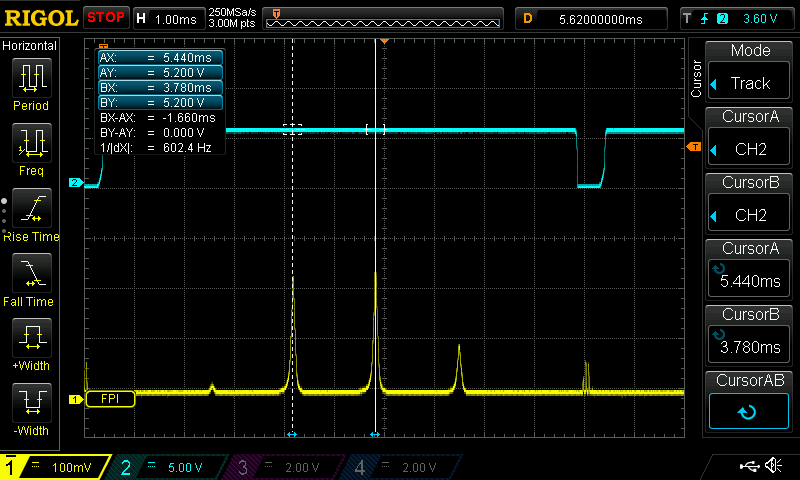
\includegraphics[width = \linewidth]{Bilder/Auswertung/FabryPerotModenAbstand.png}
    \caption{Longitudinale Lasermoden mit dem Fabry-Pérot aufgenommen. Mit den x-Markern wird der Abstand zweiter Lasermoden $\Delta \nu_{Modenabstand}$ bestimmt. Dieser muss aber noch in Hz umgerechnet werden.}
    \label{bild:AxialModenAbstand}
\end{figure}

\begin{figure}[ht]
    \centering
    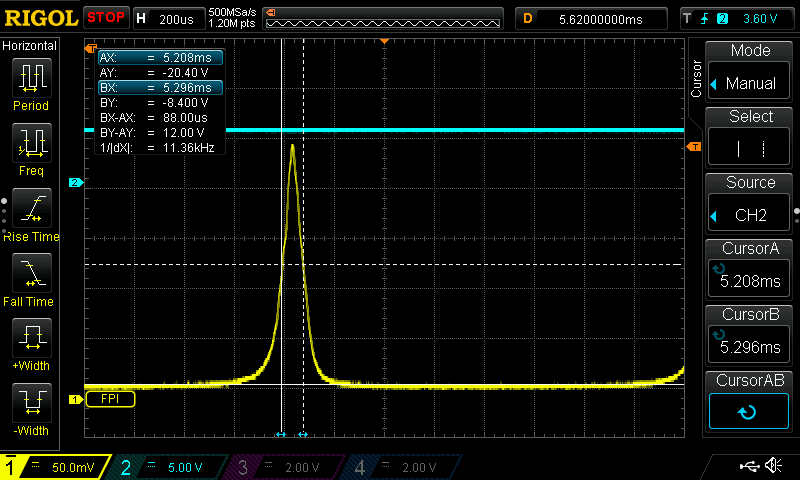
\includegraphics[width = \linewidth]{Bilder/Auswertung/FabryPerotLinienbreite.png}
    \caption{Longitudinale Lasermoden mit dem Fabry-Pérot aufgenommen. Mit den x-Markern wird die Linienbreite $\Delta \nu_{Linienbreite}$ bestimmt. Dieser muss aber noch in Hz umgerechnet werden.}
    \label{bild:Lininebreite}
\end{figure}


\begin{figure}[ht]
    \centering
    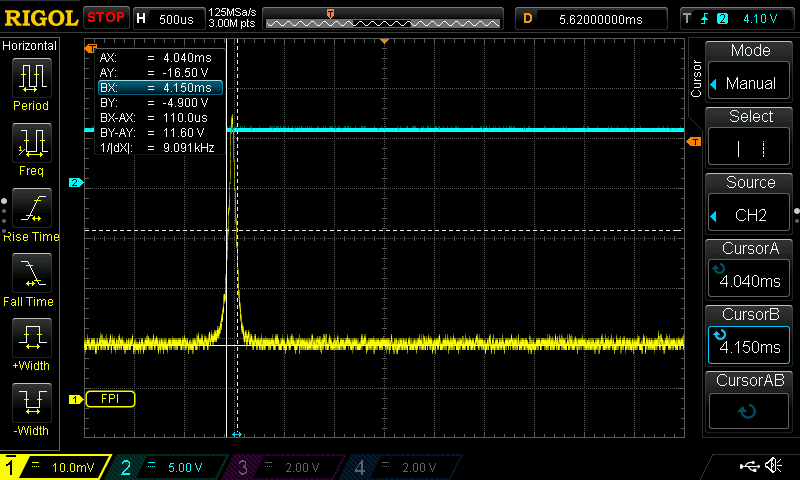
\includegraphics[width = \linewidth]{Bilder/Auswertung/FabryPerotLinienbreiteSingle.png}
    \caption{Longitudinale Lasermode mit dem Fabry-Pérot aufgenommen. Mit den x-Markern wird die Linienbreite $\Delta \nu_{Linienbreite}$ bestimmt. Dieser muss aber noch in Hz umgerechnet werden.}
    \label{bild:LininebreiteSingle}
\end{figure}

\clearpage

\section{Protokoll}

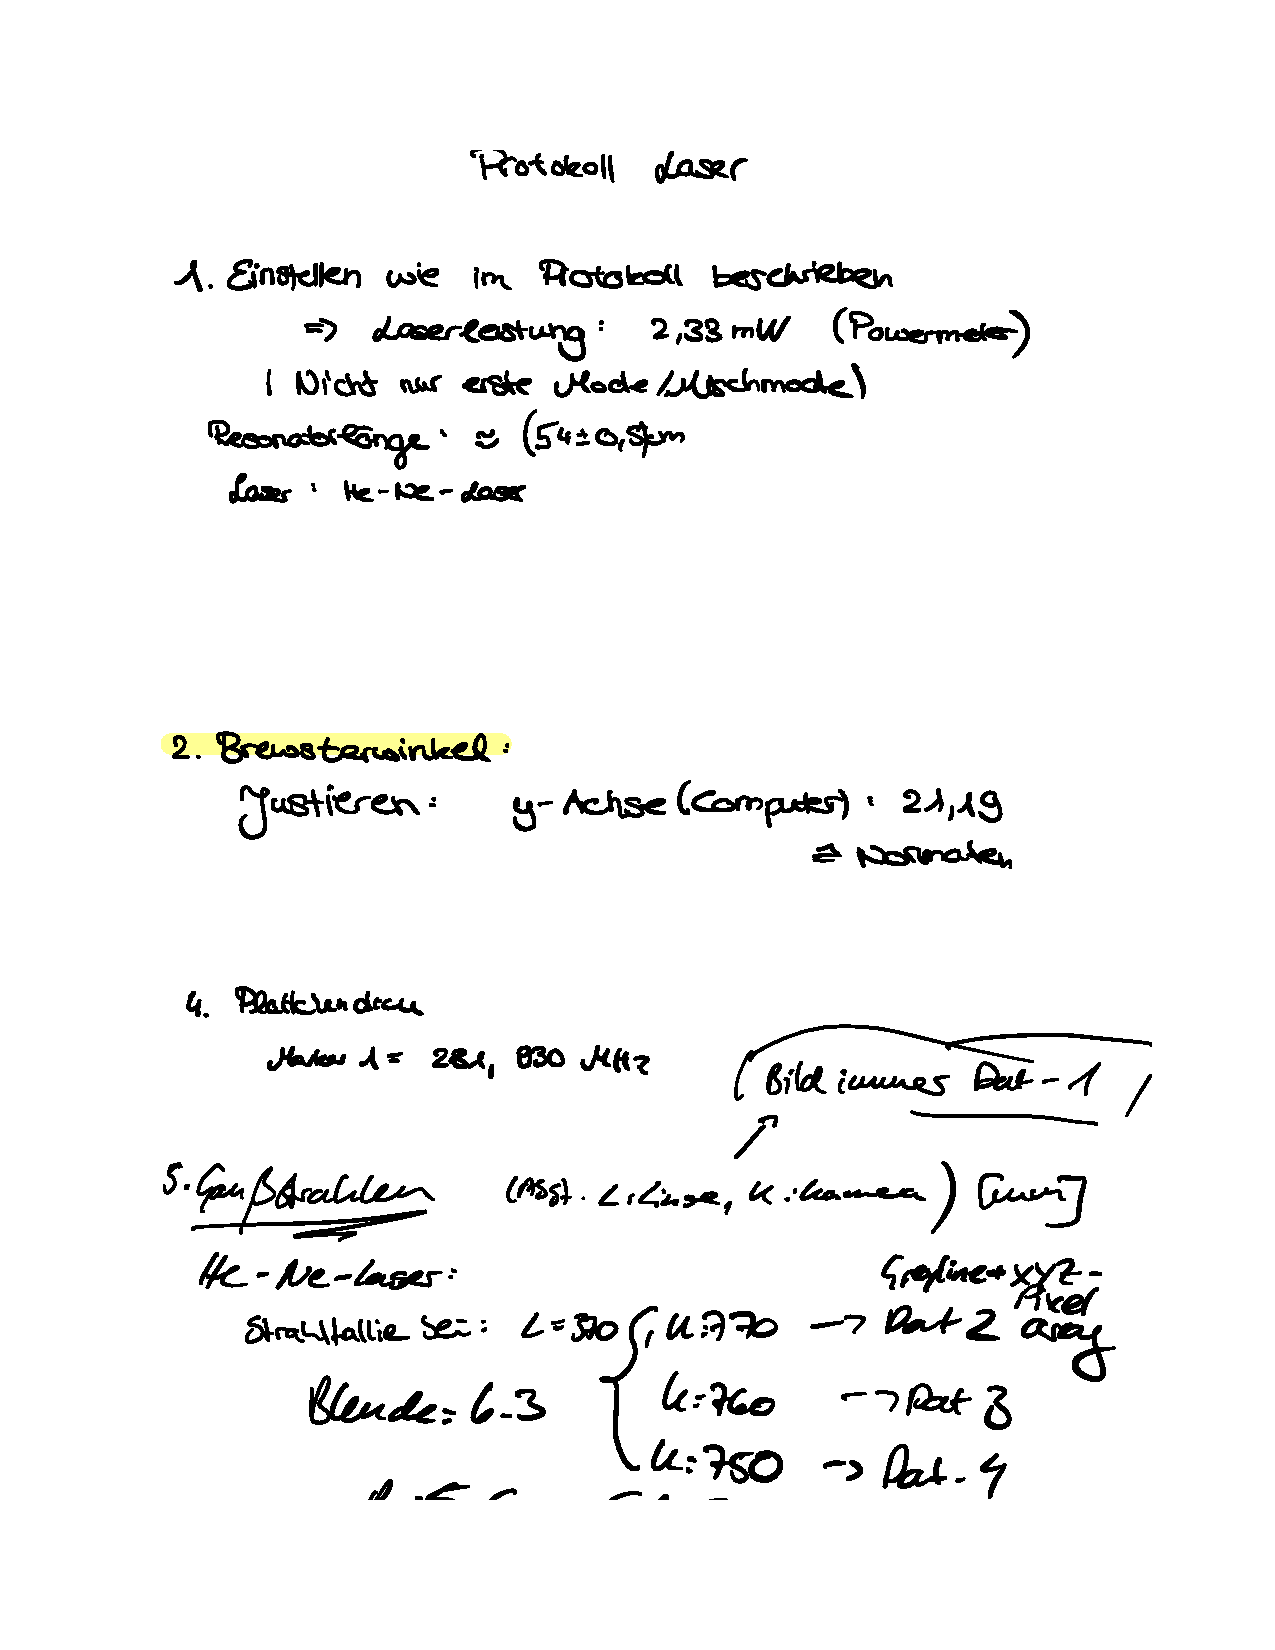
\includepdf[pages = 1-4]{LaserProt.pdf}